In this Section we introduce the Parametric Hypercubes abstract domain \adomain.

Intuitively, an abstract state of our domain tracks disjunctive information relying on floating-point intervals of fixed width. A state of \adomain\ is made by a set of hypercubes of dimension $|\variables|$. Each hypercube has $|\variables|$ sides, one for each variable, and each side contains an abstract non-relational value for the corresponding variable. Each hypercube represents a set of admissible combinations of values for all variables. 

The name Hypercubes comes from the geometric interpretation of the elements of \adomain . The concrete state of a program with variables in $\variables$ is an environment in $\funzione{\variables}{\real}$. This can be isomorphically represented by a tuple of values where each item of the tuple represents a program variable. Seen in this way, the concrete state corresponds, geometrically, to \emph{a point} in the $|\variables|$-dimensional space. Each dimension of the space represents the possible values that the corresponding variable of the program can assume. The concrete trace of a program is a sequence of points in such space (one for each state of the trace). The hypercubes of our \adomain\ domain are \emph{volumes} in the same $|\variables|$-dimensional space. Each side of the hypercube is the concretization of the abstract value of the corresponding variable, and thus it corresponds to a set of values in that dimension of the space. The concretization of an hypercube is the set of all the points contained in its volume. A state in \adomain\ is composed by a set of hypercubes: its concretization is the union of all the volumes of its hypercubes.  In this way we track disjunctive information.


\subsection{Lattice structure}
An abstract state of \adomain\ is made by a \emph{set} of hypercubes. Each hypercube is represented by a tuple of abstract values. The dimension of these tuples is equal to the number of program variables: this means that each variable is associated to a given item of the tuple (i.e., to a specific side of the hypercube). 
Consider for instance a program in which $\variables = \{x_1, x_2\}$. In this case, the hypercubes of \adomain\ are 2D-rectangles. In particular, the two sides of a single hypercube are two abstract values, one for $x_1$ and one for $x_2$.

A priori, our approach is modular w.r.t. the non-relational abstract domain we adopt to approximate the values of single variables inside an hypercube. We abstract floating-point variables through intervals of real values. We adopt set of hypercubes to improve the precision of the analysis and to track disjunctive information. This is useful, for instance, when the values of a variable are clustered in different ranges: instead of having a very big interval to cover them all (and which would cover also a lot of invalid values), we use two (or more) smaller intervals. Since it would be particularly expensive to perform all the lattice operators pointwisely, we partition the possible values into intervals of fixed width. As an example, suppose that the initial vertical velocity of the balls of our case study ranges between $50.0$ and $60.0$ or between $-60.0$ and $-50.0$. A single interval would approximate these values with $[-60.0,60.0]$, while with our approach we track two intervals, $[-60.0,-50.0]$ and $[50.0,60.0]$ (with fixed width $10.0$), which distinguish between balls thrown downwards and balls thrown upwards. The performance of this domain, though, becomes a crucial point, because the number of possible hypercubes in the space is potentially exponential with respect to the number of partitions along each spatial axis. The complexity is lightened by the use of a \emph{fixed} width for each variable, by partitioning the possible intervals, and by the efficiency of set operators on tuples.

Since a single hypercube is a tuple of intervals (one for each side), another performance booster is the use of a smart representation for intervals. In order to store the specific interval range we just use a single integer representing it. Each variable $x_i$ is associated to an interval width (specific only for that variable), which we call $w_i$ and which is a parameter of the analysis. In Section \ref{sec:tuning} we will present a variation of our analysis which computes automatically the widths, adapting them recursively and freeing the user from the need to specify values for them. For now, just notice that the smaller the width associated to a variable, the more granular and precise the analysis on that variable (and the heavier computationally the analysis). Each width $w_i$ is a floating point number that represents the width of all the possible abstract intervals associated to $x_i$. More precisely, given a width $w_i$ and an integer index $m$, the interval uniquely associated to the variable $x_i$ is $[m \times w_i, (m+1) \times w_i]$.

\textbf{Example:} Consider the case study of Section \ref{sec:case_study} and in particular the two variables \statement{px} and \statement{py}. Suppose that the widths associated to such variables are $w_1 = 10.0, w_2 = 25.0$. The hypercubes in this case are 2D-rectangles. The area of each rectangle is $10.0 \times 25.0 = 250.0$. We can draw such rectangles on the Cartesian plan, where the horizontal axis represents the values which \statement{px} can assume, and the vertical axis represents those of \statement{py}. Each side of a hypercube is identified by an integer index, representing the interval of values associated to that side. A 2D hypercube is then uniquely identified by a pair of integers. For instance, the hypercube $h_1 = ( 0, 1 )$ says that $\statement{px} \in [0.0, 10.0]$ and $\statement{py} \in [25.0, 50.0]$, while the hypercube $h_2 = ( 0, 0 )$  associates $\statement{px}$ to $[0.0, 10.0]$ and $\statement{py}$ to $[0.0, 25.0]$. In Figure \ref{fig:hcExample} we can see the graphical representation of the two hypercubes associated to the initialization of the case study (i.e., $h_1$ and $h_2$). The two axes of the Cartesian plan are split in correspondence of multiples of $10.0$ ($x$-axis) and $25.0$ ($y$-axis). In Figure \ref{fig:hcExample2}, instead, we depict the hypercubes obtained after executing the first iteration of the \statement{while} loop. Note that the hypercubes are now six. The ball is moving towards the right of the screen and is going downwards: this is coherent with the fact that the horizontal velocity is certainly positive (between $0.0$ and $60.0$), while the vertical velocity is certainly negative (between $-30.0$ and $-25.0$). 

\begin{figure}[ht]
\begin{centering}
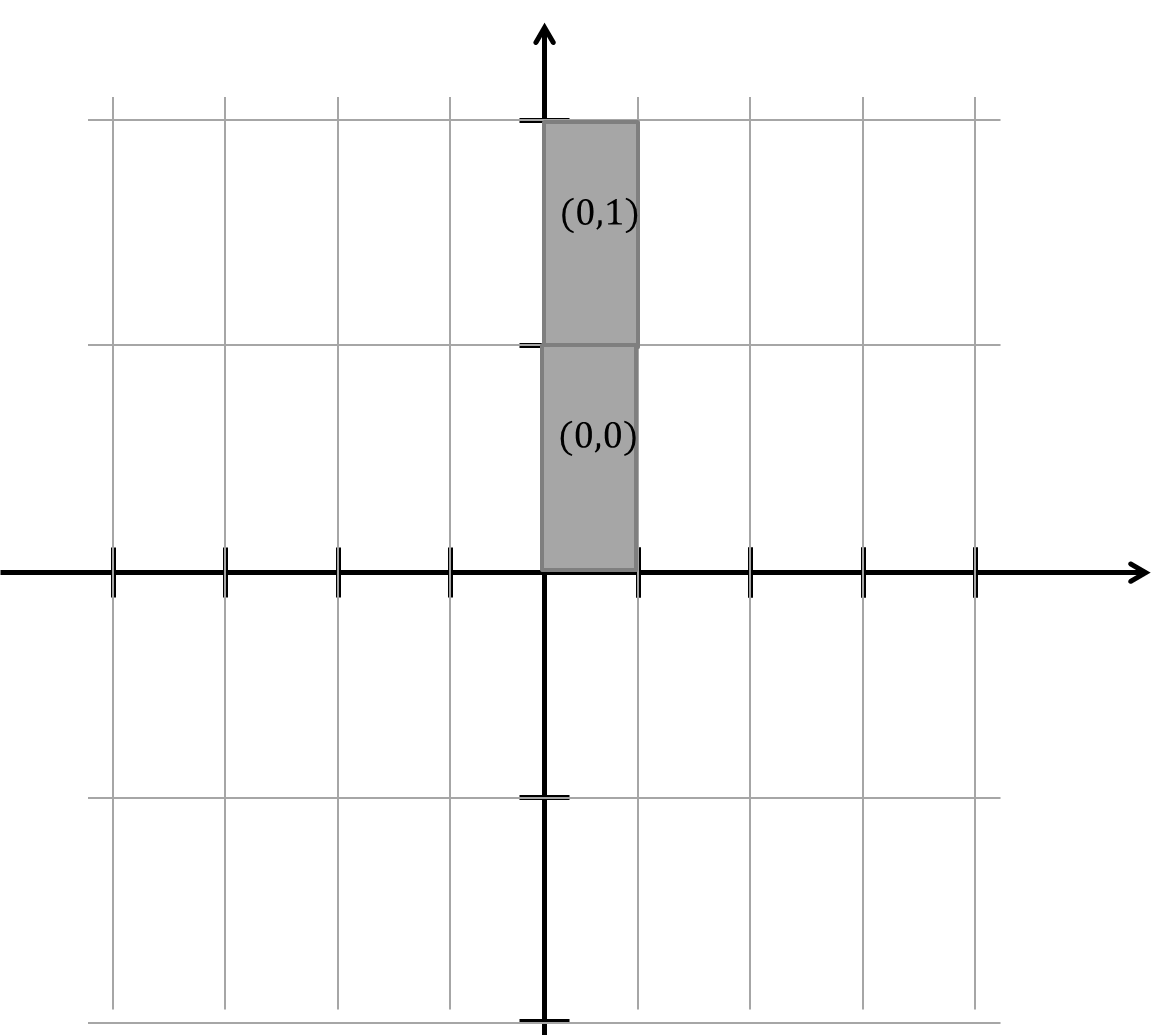
\includegraphics[scale=0.35]{Pics/example_hc_2d.png}
\caption{The abstract state of the case study after the initialization of the variables (focusing the attention only on \statement{px,py}, when their widths are, respectively, $10.0$ and $25.0$)}
\label{fig:hcExample}
\end{centering}
\end{figure}

\begin{figure}[ht]
\begin{centering}
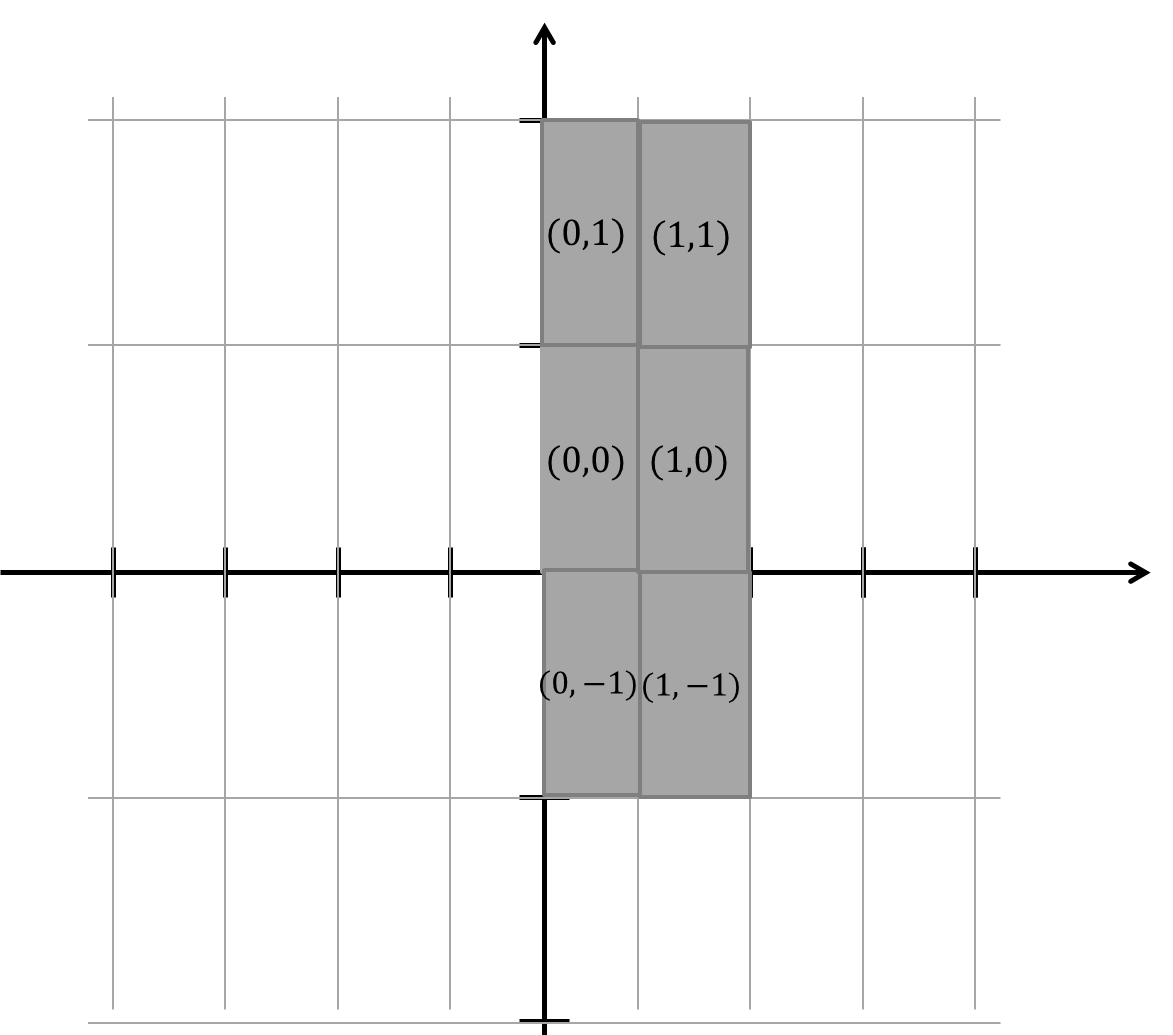
\includegraphics[scale=0.35]{Pics/example_hc_2d_2.png}
\caption{The abstract state of the case study after the first iteration of the loop (focusing the attention only on \statement{px,py}, when their widths are, respectively, $10.0$ and $25.0$)}
\label{fig:hcExample2}
\end{centering}
\end{figure}


We now define formally our abstract domain. Each abstract state is a set of hypercubes, where each hypercube is composed by $|\variables|$ integer numbers. The abstract domain is then defined by $\adomain = \wp(\integer^n)$ where $n = |\variables|$.

The definition of lattice operators relies on set operators: the partial order is defined through set inclusion, the lub and glb are set union and set intersection, respectively, while bottom and top are the empty set and the set containing all possible $n$-dimensional hypercubes, respectively. Formally, the lattice definition is $\langle\wp(\integer^n), \subseteq, \cup, \cap, \emptyset, \integer^n\rangle$.

\begin{lemma}
$\langle\wp(\integer^n), \subseteq, \cup, \cap, \emptyset, \integer^n\rangle$ is a complete lattice.
%\begin{proof}
%The proof follows immediately by basic properties of set operators.
%\end{proof}
\end{lemma}

\subsection{Concretization function}
We denote by $\ael{A}$ the non-relational abstract domain on which our analysis is parameterized, and by $n$ the number of variables of the program, where $n = | \variables |$.

$$
\begin{array}{l}
\gamma_{\aval} : \funzione{\wp(\integer^n)}{\wp(\real^\variables)}\\
\gamma_{\aval}(\ael{V}) = \{\sigma : \exists v \in \ael{V} : \forall i \in [1..n] : \sigma_i \in \gamma_\ael{A}(\afunction{getAbsValue}_v(i)) \}
\end{array}
$$

where: (i) $\sigma \in \real^\variables$ and $\sigma_i \in \real$ denotes the $i$-th element of the tuple $\sigma$, (ii) $\gamma_\ael{A} : \funzione{\ael{A}}{\wp(\real)}$ is the concretization function of abstract values of the non-relational abstract domain on which our analysis is parameterized, and (iii)  $\afunction{getAbsValue}_v : \funzione{\naturals}{\ael{A}}$ is the function that, given an integer index, returns the abstract value (in the domain $\ael{A}$) which corresponds to that index inside the tuple $v$.

$\gamma_{\aval}$ concretizes a set of hypercubes to a set of vectors of $n$ floating point values. 

$$
\begin{array}{l}
\gamma_{\adomain} : \funzione{\wp(\integer^n)}{\wp(\funzione{\variables}{\real})}\\
\gamma_{\adomain}(\ael{V}) = \{[\statement{x} \mapsto \cel{r}(\avariableindex{\statement{x}}) : \statement{x} \in \variables] : \cel{r} \in \gamma_{\aval}(\ael{V})\}
\end{array}
$$

$\gamma_{\adomain}$ simply transforms the vectors returned by $\gamma_{\aval}$ into concrete environments relying on the function $\avariableindexname : \funzione{\variables}{\naturals}$, that, given a variable, returns its index in the elements of \adomain.

%Intuitively, we represent a concrete value as a tuple of real values (one for each variable of the program). The concretization of an abstract state $h \in \adomain$ is then a set of tuples. The concretization of $h$ is the union of all the concretizations of its hypercubes, i.e., all the points belonging to the volumes of its hypercubes. Each tuple of the concretization of $h$, then, is a point belonging to one hypercube of $h$. 

\subsection{Widening operator}
The domain described so far does not ensure the convergence of the analysis. In fact, a \statement{while} loop may add new hypercubes with increased indices at each iteration, and the dimension of the abstract state (i.e., the hypercubes set) would increase at each iteration without converging. Thus, we need a way to force the convergence of the analysis. Given our abstract state representation, we fix for each variable of the program a maximum integer index $n_i$ such that $n_i$ represents the interval $[n_i \times w_i, +\infty]$. The same happens symmetrically for negative values. In this way, the set of indices of a given variable is finite, and the resulting domain has finite height. Thus, in this scenario, the widening operator coincides with the lub operator, i.e., set union. 

This approach may seem too rough since we establish the bounds of intervals before running the analysis. However, this allows us to control the number of possible intervals in our hypercubes, and this is particularly important for the efficiency of the overall analysis. In addition, when analysing physics simulations we can use the initialization of variables and the property we want to check in order to establish convenient bounds for the intervals. For instance, in the case study presented in Section \ref{sec:case_study} we are interested in checking if a ball stays in the screen, that is, if \statement{px} is greater than zero and less than a given value \statement{w} representing the width of the screen.

Observe that more sophisticated widening operators could be used as an alternative to the adopted solution described above, but this could affect the performance of the resulting analysis.

%\subsection{Other data types or non-relational abstractions}
%\todogiulia{Secondo me questa subsection si puo' cancellare}
%As suggested before, for now we focus the application of our abstract domain to physics simulations, and for this reason we abstract floating point variables through intervals of fixed width. However, we may apply other kind of abstractions (e.g., the Sign domain) to our framework to consider other types of variables (integer, boolean, etc.). We will sketch other possible applications of our framework in Section \ref{sec:otherapplications}.

